\section{Visualization I}
Let's pick a few simple matrices and look at a representation of their \svdl s.

\break
\clearpage
%%%
\section{Building low rank objects}
The simple objects are a natural starting point for we can probe the simplest cases analytically and then turn to numeric treatment for more elaborate examples. Also, it helps to look at objects that are flat or smooth or pointed. The first objects we examine will have low matrix rank.

%%
\subsection{The triangle}
The first object we construct will be a triangle. In the continuum limit we will see a sharp point at the apex and smooth sides.
\begin{table}[htdp]
\begin{center}
\begin{tabular}{lcc}
  1 & $\mat{ccc}{0&0&0\\0&1&0\\0&0&0}$ & 
  \includegraphics[ width = 1.5in ]{pdf/"ch 08"/triangle/triangle_001} \\
  2 & $\mat{ccccc}{0&0&0&0&0\\0&0&1&0&0\\0&1&1&1&0\\0&0&0&0&0}$ & 
  \includegraphics[ width = 1.5in ]{pdf/"ch 08"/triangle/triangle_002} \\
  3 & $\mat{ccccccc}{0&0&0&0&0&0&0\\0&0&0&1&0&0&0\\0&0&1&1&1&0&0\\0&1&1&1&1&1&0\\0&0&0&0&0&0&0}$ & \includegraphics[ width = 1.5in ]{pdf/"ch 08"/triangle/triangle_003} \\
  4 & $\mat{ccccccccc}{0&0&0&0&0&0&0&0&0\\0&0&0&0&1&0&0&0&0\\0&0&0&1&1&1&0&0&0\\0&0&1&1&1&1&1&0&0\\0&1&1&1&1&1&1&1&0\\0&0&0&0&0&0&0&0&0}$ & 
  \includegraphics[ width = 1.5in ]{pdf/"ch 08"/triangle/triangle_004} \\
\end{tabular}
\end{center}
\label{tab:triangles}
\caption{default}
\end{table}%

Consider the triangle shown in table \eqref{tab:triangles}. The first matrix is given by this
\begin{equation}
  \A{} = \mat{c|c|c}{0&0&0\\0&1&0\\0&0&0}.
\end{equation}
We see that the column space has two independent vectors
\begin{equation}
  c_{1} = \A{}_{*,1} = \mat{c}{0\\0\\0}, \quad c_{2} = \A{}_{*,2} = \mat{c}{0\\1\\0}.
\end{equation}
The third column is a copy of the first column
\begin{equation}
  c_{3} = \A{}_{*,2} = \A{}_{*,1} = c_{1}.
\end{equation}

From this we conclude that the matrix $\A{}$ has rank $\rho=1$. We have now specified the problem and can identify the structure of the decomposition. We can perform SVD by inspection.

Because the target matrix has $m=3$ rows, the codomain matrix $\Y{}$ will be a 3 $\times$ 3 matrix. Because the target matrix has rank $\rho=1$, there is one range vector and $m-\rho=2$ null space vectors.

Because the target matrix has $n=3$ columns, the domain matrix $\X{}$ will be a 3 $\times$ 3 matrix. Because the target matrix has rank $\rho=1$, there is one range vectors and $m-\rho=2$ null space vectors.

The first guess for the domain matrices involves trying the unit vectors:
\begin{equation}
  \Y{} = \mat{c>{\columncolor{ltgray}}c>{\columncolor{ltgray}}c}{0&1&0\\1&0&0\\0&0&1}, \quad
  \X{} = \mat{c>{\columncolor{ltgray}}c>{\columncolor{ltgray}}c}{0&1&0\\1&0&0\\0&0&1}.
\end{equation}
From this we see that the matrix of singular values is given by this:
\begin{equation}
  \sig{} = \mat{ccc}{1&0&0\\0&0&0\\0&0&0}.
\end{equation}

Consider the triangle shown in table \eqref{tab:triangles}. The first matrix is given by this
\begin{equation}
  \A{} = \mat{c|c|c}{0&0&0\\0&1&0\\0&0&0}.
\end{equation}
We see that the column space has two independent vectors
\begin{equation}
  c_{1} = \A{}_{*,1} = \mat{c}{0\\0\\0}, \quad c_{2} = \A{}_{*,2} = \mat{c}{0\\1\\0}.
\end{equation}
The third column is a copy of the first column
\begin{equation}
  c_{3} = \A{}_{*,2} = \A{}_{*,1} = c_{1}.
\end{equation}

Observe the shapes of the different matrices and look at the form for the $\sig{}$ matrix. The domain matrices show interesting patterns for the image and kernels. The circle is a low rank object. 
%%%

\break
\clearpage

%\begin{table}[htdp]
%\begin{center}
%\begin{tabular}{ccccc}
% && $\Y{}$ & $\sig{}$ & $\X{}$ \\
%\includegraphics[ width = 1in ]{pdf/"ch 08"/triangle/triangle_00001_A} &&
%\includegraphics[ width = 1in ]{pdf/"ch 08"/triangle/triangle_00001_Y} &
%\includegraphics[ width = 1in ]{pdf/"ch 08"/triangle/triangle_00001_S} &
%\includegraphics[ width = 1in ]{pdf/"ch 08"/triangle/triangle_00001_Xt} \\[5pt]
%%%%
%\includegraphics[ width = 1in ]{pdf/"ch 08"/triangle/triangle_00002_A} &&
%\includegraphics[ width = 1in ]{pdf/"ch 08"/triangle/triangle_00002_Y} 
%\includegraphics[ width = 1in ]{pdf/"ch 08"/triangle/triangle_00002_S} 
%\includegraphics[ width = 1in ]{pdf/"ch 08"/triangle/triangle_00002_Xt} \\[5pt]
%%%%
%\includegraphics[ width = 1in ]{pdf/"ch 08"/triangle/triangle_00003_A} &&
%\includegraphics[ width = 1in ]{pdf/"ch 08"/triangle/triangle_00003_Y} 
%\includegraphics[ width = 1in ]{pdf/"ch 08"/triangle/triangle_00003_S} 
%\includegraphics[ width = 1in ]{pdf/"ch 08"/triangle/triangle_00003_Xt} \\[5pt]
%%%%
%\includegraphics[ width = 1in ]{pdf/"ch 08"/triangle/triangle_00005_A} &&
%\includegraphics[ width = 1in ]{pdf/"ch 08"/triangle/triangle_00005_Y} 
%\includegraphics[ width = 1in ]{pdf/"ch 08"/triangle/triangle_00005_S} 
%\includegraphics[ width = 1in ]{pdf/"ch 08"/triangle/triangle_00005_Xt} \\[5pt]
%%%%
%\includegraphics[ width = 1in ]{pdf/"ch 08"/triangle/triangle_00010_A} &&
%\includegraphics[ width = 1in ]{pdf/"ch 08"/triangle/triangle_00010_Y} 
%\includegraphics[ width = 1in ]{pdf/"ch 08"/triangle/triangle_00010_S} 
%\includegraphics[ width = 1in ]{pdf/"ch 08"/triangle/triangle_00010_Xt} \\[5pt]
%%%%
%\includegraphics[ width = 1in ]{pdf/"ch 08"/triangle/triangle_00020_A} &&
%\includegraphics[ width = 1in ]{pdf/"ch 08"/triangle/triangle_00020_Y} 
%\includegraphics[ width = 1in ]{pdf/"ch 08"/triangle/triangle_00020_S} 
%\includegraphics[ width = 1in ]{pdf/"ch 08"/triangle/triangle_00020_Xt} \\
%%%%
%%%%
%\end{tabular}
%\end{center}
%\label{fourier:triangle:SVDpictures}
%\caption[The \svdl \ for the triangle]{The \svdl \ for the triangle. Observe the shapes of the different matrices and look at the form for the $\sig{}$ matrix. The domain matrices show interesting patterns for the image and kernels. The triangle rank saturates as the size increases.}
%\end{table}%
%%%%%%%%%%%%%

\begin{table}[htdp]
\begin{center}
\begin{tabular}{ccccc}
 \titlea \\
\includegraphics[ width = 1in ]{pdf/"ch 08"/disk/bw_0003_A} &&
\includegraphics[ width = 1in ]{pdf/"ch 08"/disk/bw_0003_Y} &
\includegraphics[ width = 1in ]{pdf/"ch 08"/disk/bw_0003_S} &
\includegraphics[ width = 1in ]{pdf/"ch 08"/disk/bw_0003_Xt} \\[5pt]
%%%
\includegraphics[ width = 1in ]{pdf/"ch 08"/disk/bw_0005_A} &&
\includegraphics[ width = 1in ]{pdf/"ch 08"/disk/bw_0005_Y} &
\includegraphics[ width = 1in ]{pdf/"ch 08"/disk/bw_0005_S} &
\includegraphics[ width = 1in ]{pdf/"ch 08"/disk/bw_0005_Xt} \\[5pt]
%%%

\includegraphics[ width = 1in ]{pdf/"ch 08"/disk/bw_0010_A} &&
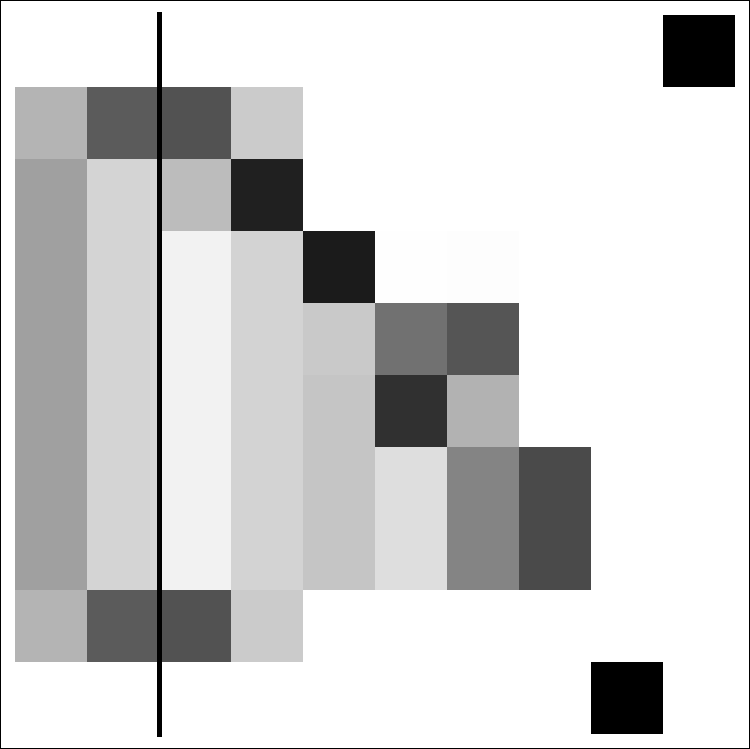
\includegraphics[ width = 1in ]{pdf/"ch 08"/disk/bw_0010_Y} &

\includegraphics[ width = 1in ]{pdf/"ch 08"/disk/bw_0010_S} &
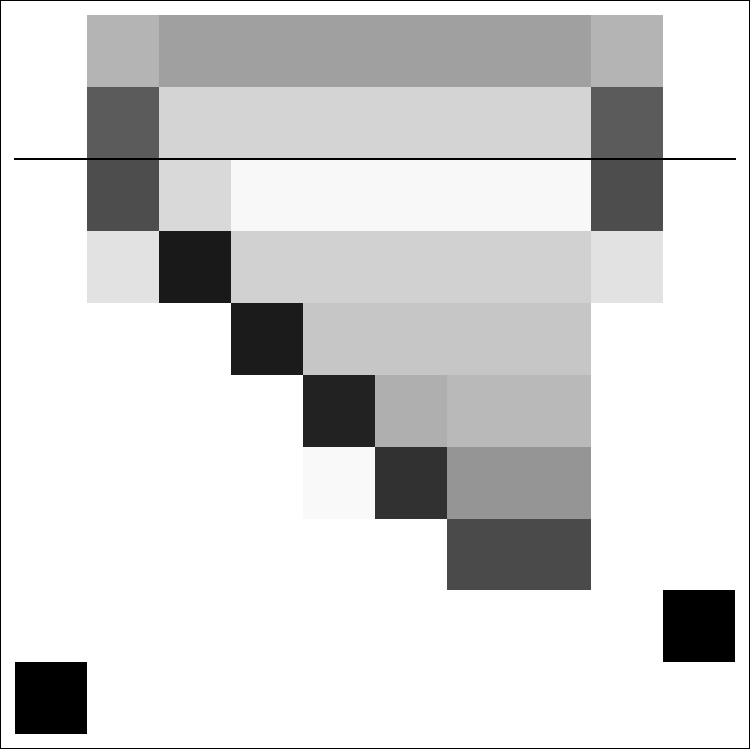
\includegraphics[ width = 1in ]{pdf/"ch 08"/disk/bw_0010_Xt} \\[5pt]
%%%
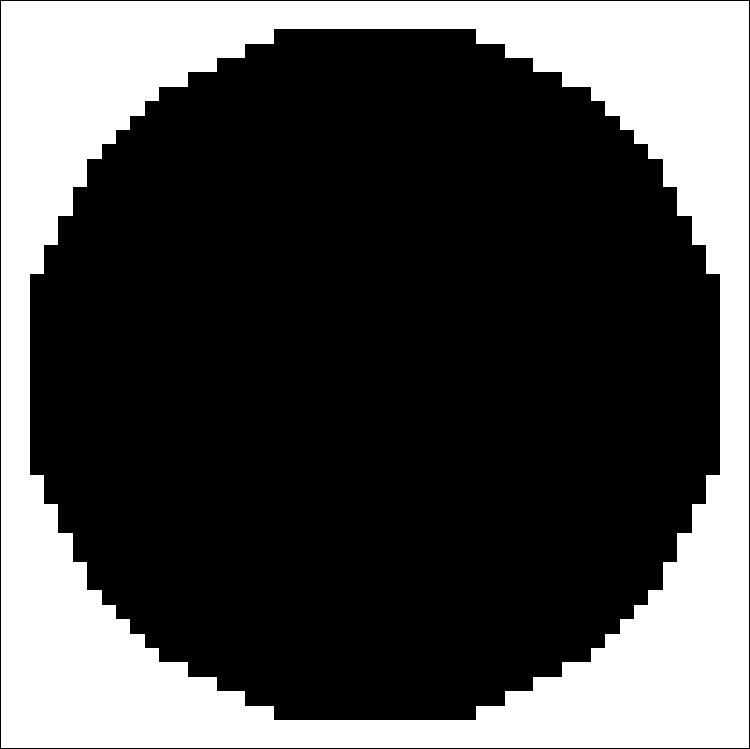
\includegraphics[ width = 1in ]{pdf/"ch 08"/disk/bw_0050_A} &&
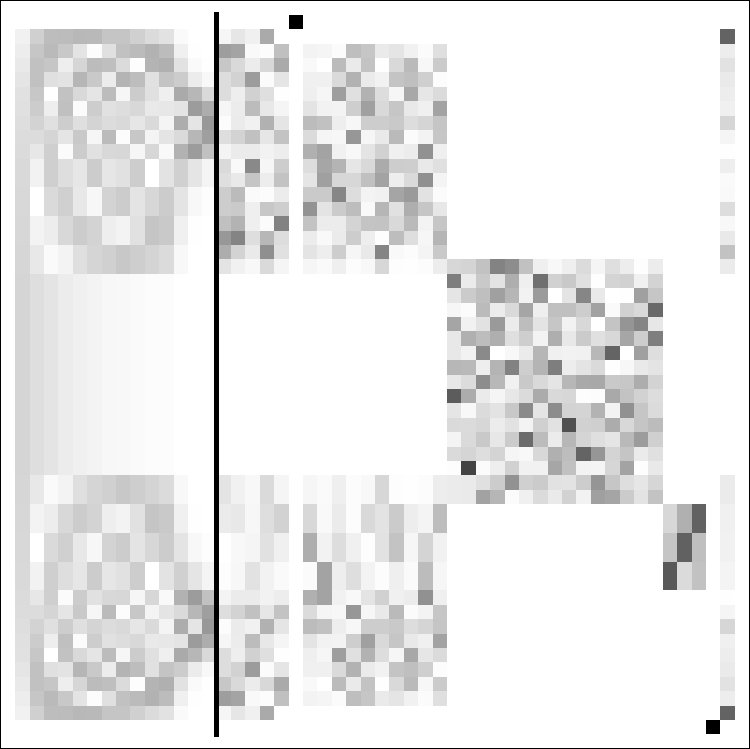
\includegraphics[ width = 1in ]{pdf/"ch 08"/disk/bw_0050_Y} &

\includegraphics[ width = 1in ]{pdf/"ch 08"/disk/bw_0050_S} &
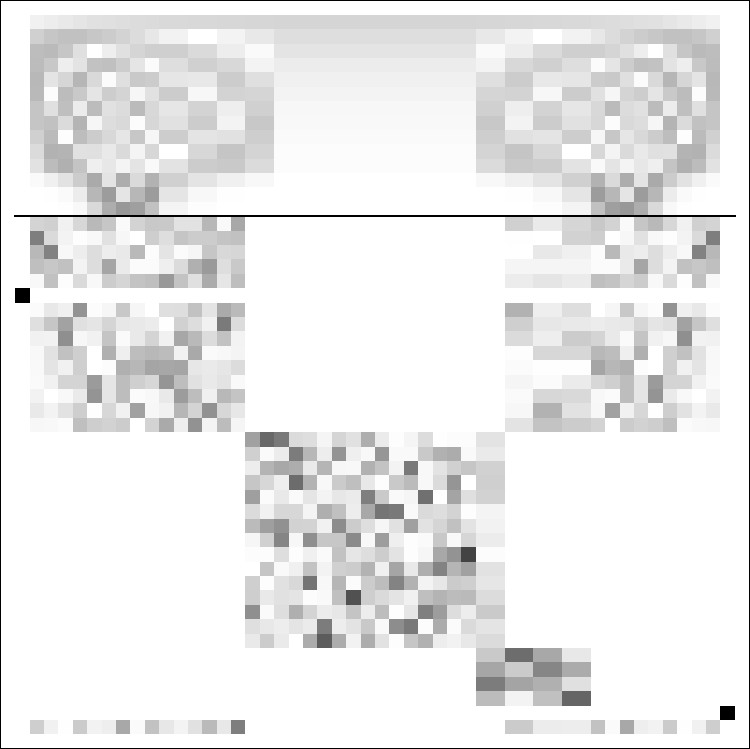
\includegraphics[ width = 1in ]{pdf/"ch 08"/disk/bw_0050_Xt} \\[5pt]
%%%
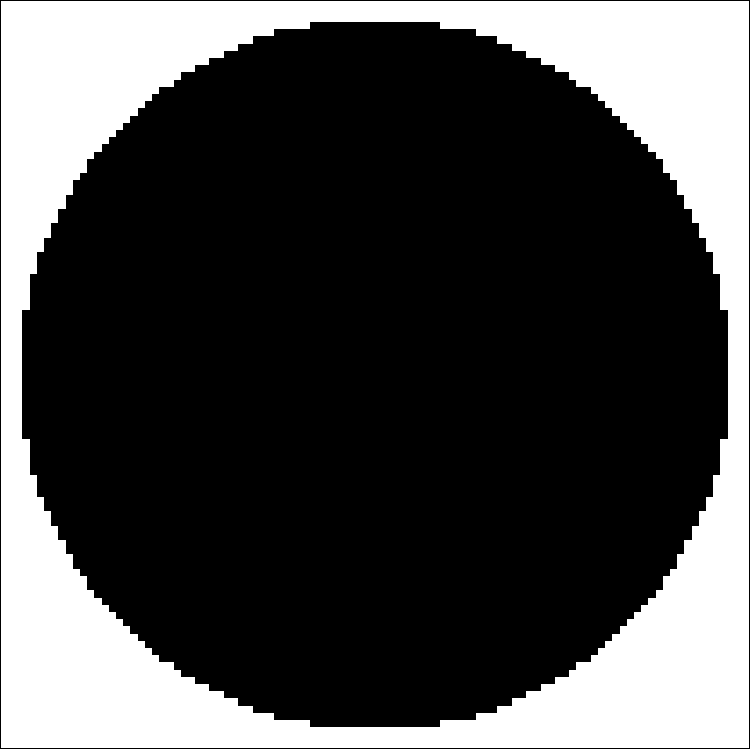
\includegraphics[ width = 1in ]{pdf/"ch 08"/disk/bw_0100_A} &&
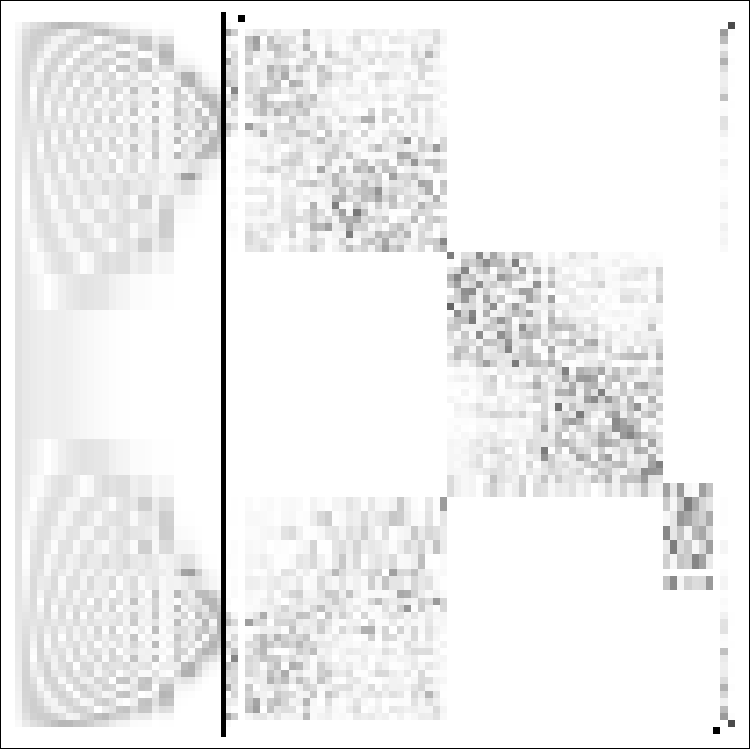
\includegraphics[ width = 1in ]{pdf/"ch 08"/disk/bw_0100_Y} &
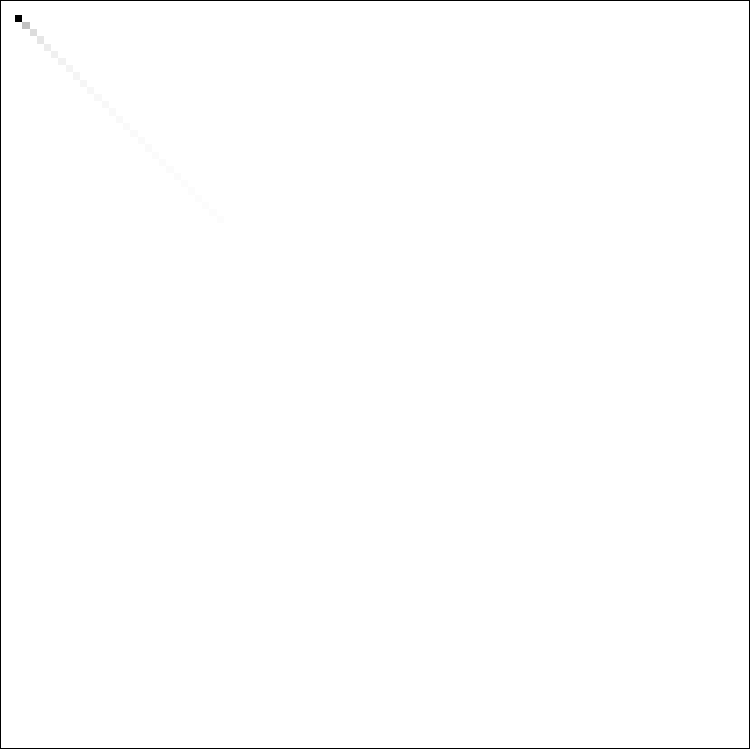
\includegraphics[ width = 1in ]{pdf/"ch 08"/disk/bw_0100_S} &
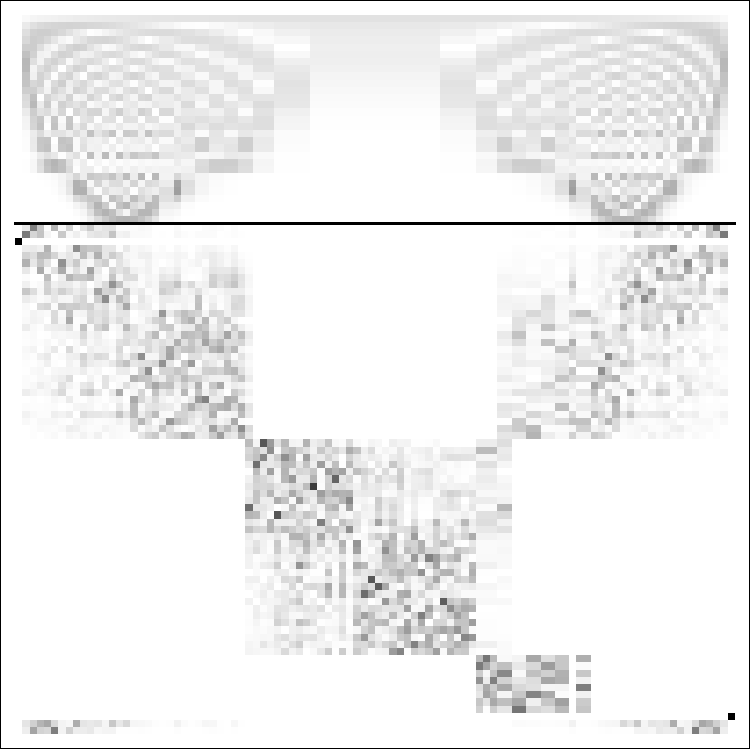
\includegraphics[ width = 1in ]{pdf/"ch 08"/disk/bw_0100_Xt} \\[5pt]
%%%
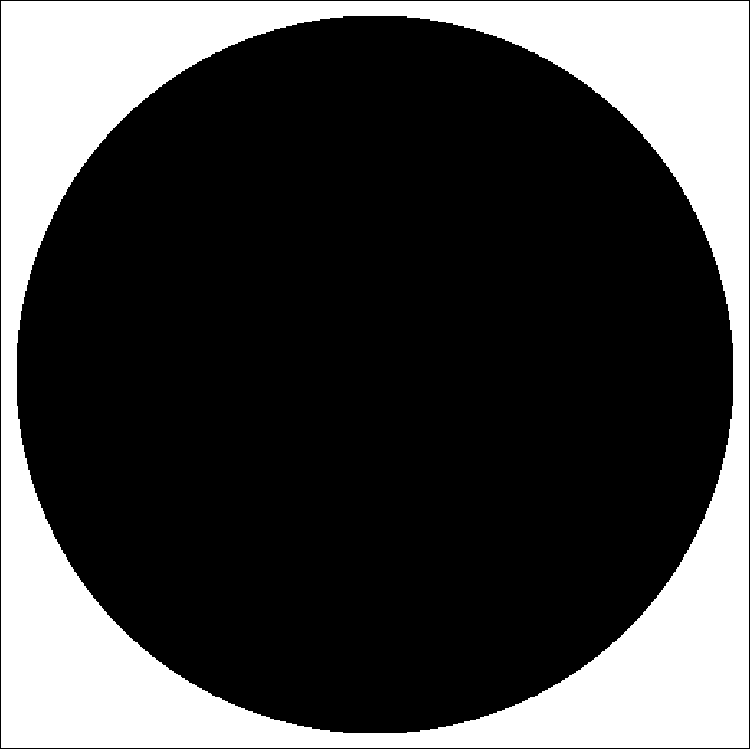
\includegraphics[ width = 1in ]{pdf/"ch 08"/disk/bw_0500_A} &&
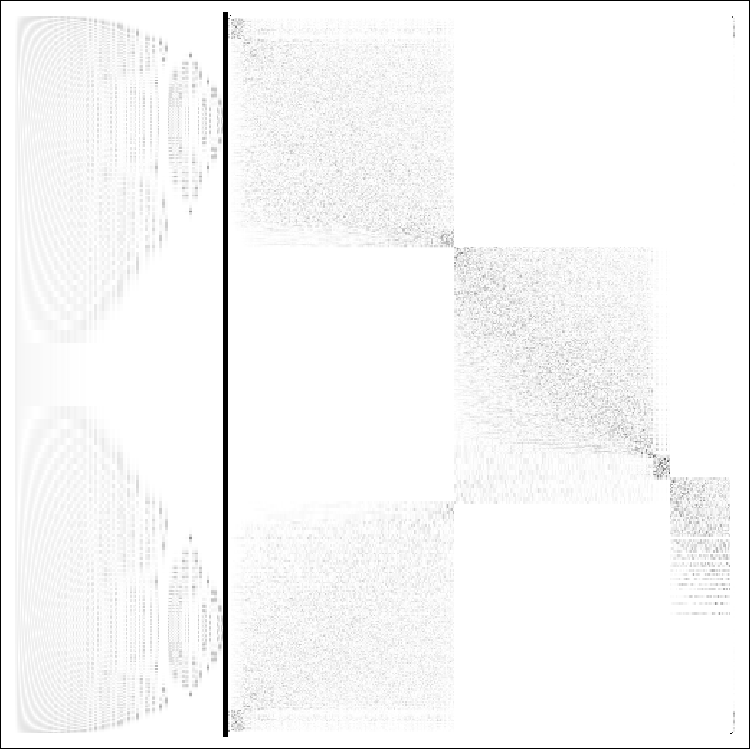
\includegraphics[ width = 1in ]{pdf/"ch 08"/disk/bw_0500_Y} &
\includegraphics[ width = 1in ]{pdf/"ch 08"/disk/bw_0500_S} &
\includegraphics[ width = 1in ]{pdf/"ch 08"/disk/bw_0500_Xt} \\
%%%
%%%
\end{tabular}
\end{center}
\label{fourier:disk:SVDpictures}
\caption[The \svdl \ for the disk]{The \svdl \ for the disk. The matrices are square and have dimensions $n=3,5,10,50,100,500$.}
\end{table}%

%%%%%%%%%%%%
\begin{table}[htdp]
\begin{center}
\begin{tabular}{ccccc}
 \titlea \\
%%%
\includegraphics[ width = 1in ]{pdf/"ch 08"/dither/disk_dither_0003_A} &&
\includegraphics[ width = 1in ]{pdf/"ch 08"/dither/disk_dither_0003_Y} &
\includegraphics[ width = 1in ]{pdf/"ch 08"/dither/disk_dither_0003_S} &
\includegraphics[ width = 1in ]{pdf/"ch 08"/dither/disk_dither_0003_Xt} \\[5pt]
%%%
\includegraphics[ width = 1in ]{pdf/"ch 08"/dither/disk_dither_0005_A} &&
\includegraphics[ width = 1in ]{pdf/"ch 08"/dither/disk_dither_0005_Y} &
\includegraphics[ width = 1in ]{pdf/"ch 08"/dither/disk_dither_0005_S} &
\includegraphics[ width = 1in ]{pdf/"ch 08"/dither/disk_dither_0005_Xt} \\[5pt]
%%%
\includegraphics[ width = 1in ]{pdf/"ch 08"/dither/disk_dither_0010_A} &&
\includegraphics[ width = 1in ]{pdf/"ch 08"/dither/disk_dither_0010_Y} &
\includegraphics[ width = 1in ]{pdf/"ch 08"/dither/disk_dither_0010_S} &
\includegraphics[ width = 1in ]{pdf/"ch 08"/dither/disk_dither_0010_Xt} \\[5pt]
%%%
\includegraphics[ width = 1in ]{pdf/"ch 08"/dither/disk_dither_0050_A} &&
\includegraphics[ width = 1in ]{pdf/"ch 08"/dither/disk_dither_0050_Y} &
\includegraphics[ width = 1in ]{pdf/"ch 08"/dither/disk_dither_0050_S} &
\includegraphics[ width = 1in ]{pdf/"ch 08"/dither/disk_dither_0050_Xt} \\[5pt]
%%%
\includegraphics[ width = 1in ]{pdf/"ch 08"/dither/disk_dither_0100_A} &&
\includegraphics[ width = 1in ]{pdf/"ch 08"/dither/disk_dither_0100_Y} &
\includegraphics[ width = 1in ]{pdf/"ch 08"/dither/disk_dither_0100_S} &
\includegraphics[ width = 1in ]{pdf/"ch 08"/dither/disk_dither_0100_Xt} \\[5pt]
%%%
\includegraphics[ width = 1in ]{pdf/"ch 08"/dither/disk_dither_0500_A} &&
\includegraphics[ width = 1in ]{pdf/"ch 08"/dither/disk_dither_0500_Y} &
\includegraphics[ width = 1in ]{pdf/"ch 08"/dither/disk_dither_0500_S} &
\includegraphics[ width = 1in ]{pdf/"ch 08"/dither/disk_dither_0500_Xt} \\
%%%
\end{tabular}
\end{center}
\label{fourier:disk:SVDpictures}
\caption[The \svdl \ for the dithered disk]{The \svdl \ for the dithered disk. The matrices are square and have the same dimensions as in the previous table: dimensions $n=3,5,10,50,100,500$.}
\end{table}%

%%%%%%%%%%%%
\begin{table}[htdp]
\begin{center}
\begin{tabular}{ccccc}
 \titlea \\
%%%
\includegraphics[ width = 1in ]{pdf/"ch 08"/ring/ring_0003_A} &&
\includegraphics[ width = 1in ]{pdf/"ch 08"/ring/ring_0003_Y} &
\includegraphics[ width = 1in ]{pdf/"ch 08"/ring/ring_0003_S} &
\includegraphics[ width = 1in ]{pdf/"ch 08"/ring/ring_0003_Xt} \\[5pt]
%%%
\includegraphics[ width = 1in ]{pdf/"ch 08"/ring/ring_0010_A} &&
\includegraphics[ width = 1in ]{pdf/"ch 08"/ring/ring_0010_Y} &
\includegraphics[ width = 1in ]{pdf/"ch 08"/ring/ring_0010_S} &
\includegraphics[ width = 1in ]{pdf/"ch 08"/ring/ring_0010_Xt} \\[5pt]
%%%
\includegraphics[ width = 1in ]{pdf/"ch 08"/ring/ring_0050_A} &&
\includegraphics[ width = 1in ]{pdf/"ch 08"/ring/ring_0050_Y} &
\includegraphics[ width = 1in ]{pdf/"ch 08"/ring/ring_0050_S} &
\includegraphics[ width = 1in ]{pdf/"ch 08"/ring/ring_0050_Xt} \\[5pt]
%%%
\includegraphics[ width = 1in ]{pdf/"ch 08"/ring/ring_0100_A} &&
\includegraphics[ width = 1in ]{pdf/"ch 08"/ring/ring_0100_Y} &
\includegraphics[ width = 1in ]{pdf/"ch 08"/ring/ring_0100_S} &
\includegraphics[ width = 1in ]{pdf/"ch 08"/ring/ring_0100_Xt} \\[5pt]
%%%
\includegraphics[ width = 1in ]{pdf/"ch 08"/ring/ring_0500_A} &&
\includegraphics[ width = 1in ]{pdf/"ch 08"/ring/ring_0500_Y} &
\includegraphics[ width = 1in ]{pdf/"ch 08"/ring/ring_0500_S} &
\includegraphics[ width = 1in ]{pdf/"ch 08"/ring/ring_0500_Xt} \\
%%%
\includegraphics[ width = 1in ]{pdf/"ch 08"/ring/ring_1000_A} &&
\includegraphics[ width = 1in ]{pdf/"ch 08"/ring/ring_1000_Y} &
\includegraphics[ width = 1in ]{pdf/"ch 08"/ring/ring_1000_S} &
\includegraphics[ width = 1in ]{pdf/"ch 08"/ring/ring_1000_Xt} \\[5pt]
%%%
\end{tabular}
\end{center}
\label{fourier:disk:SVDpictures}
\caption[The \svdl \ for the ring]{The \svdl \ for the ring. The matrices are square and have the same dimensions as in the previous table: dimensions $n=3,10,50,100,500,1000$.}
\end{table}%

%%%%%%%%%%%%  ramp
\begin{table}[htdp]
\begin{center}
\begin{tabular}{ccccc}
 \titlea \\
%%%
\includegraphics[ width = 1in ]{pdf/"ch 08"/ramp/ramp_0002_A} &&
\includegraphics[ width = 1in ]{pdf/"ch 08"/ramp/ramp_0002_Y} &
\includegraphics[ width = 1in ]{pdf/"ch 08"/ramp/ramp_0002_S} &
\includegraphics[ width = 1in ]{pdf/"ch 08"/ramp/ramp_0002_Xt} \\[5pt]
%%%
\includegraphics[ width = 1in ]{pdf/"ch 08"/ramp/ramp_0005_A} &&
\includegraphics[ width = 1in ]{pdf/"ch 08"/ramp/ramp_0005_Y} &
\includegraphics[ width = 1in ]{pdf/"ch 08"/ramp/ramp_0005_S} &
\includegraphics[ width = 1in ]{pdf/"ch 08"/ramp/ramp_0005_Xt} \\[5pt]
%%%
\includegraphics[ width = 1in ]{pdf/"ch 08"/ramp/ramp_0010_A} &&
\includegraphics[ width = 1in ]{pdf/"ch 08"/ramp/ramp_0010_Y} &
\includegraphics[ width = 1in ]{pdf/"ch 08"/ramp/ramp_0010_S} &
\includegraphics[ width = 1in ]{pdf/"ch 08"/ramp/ramp_0010_Xt} \\[5pt]
%%%
\includegraphics[ width = 1in ]{pdf/"ch 08"/ramp/ramp_0020_A} &&
\includegraphics[ width = 1in ]{pdf/"ch 08"/ramp/ramp_0020_Y} &
\includegraphics[ width = 1in ]{pdf/"ch 08"/ramp/ramp_0020_S} &
\includegraphics[ width = 1in ]{pdf/"ch 08"/ramp/ramp_0020_Xt} \\[5pt]
%%%
\includegraphics[ width = 1in ]{pdf/"ch 08"/ramp/ramp_0050_A} &&
\includegraphics[ width = 1in ]{pdf/"ch 08"/ramp/ramp_0050_Y} &
\includegraphics[ width = 1in ]{pdf/"ch 08"/ramp/ramp_0050_S} &
\includegraphics[ width = 1in ]{pdf/"ch 08"/ramp/ramp_0050_Xt} \\[5pt]
%%%
\includegraphics[ width = 1in ]{pdf/"ch 08"/ramp/ramp_0100_A} &&
\includegraphics[ width = 1in ]{pdf/"ch 08"/ramp/ramp_0100_Y} &
\includegraphics[ width = 1in ]{pdf/"ch 08"/ramp/ramp_0100_S} &
\includegraphics[ width = 1in ]{pdf/"ch 08"/ramp/ramp_0100_Xt} \\[5pt]
%%%
\end{tabular}
\end{center}
\label{fourier:disk:SVDpictures}
\caption[The \svdl \ for the ramp]{The \svdl \ for the ramp. The matrices are square and have the same dimensions as in the previous table: dimensions $n=2,5,10,20,50,100$.}
\end{table}%

%%%%%%%%%%%%  TONES ALPHA
\begin{table}[htdp]
\begin{center}
\begin{tabular}{ccccc}
 \titlea \\
%%%
\includegraphics[ width = 1in ]{pdf/"ch 08"/tones_alpha/tones_alpha_0002_A} &&
\includegraphics[ width = 1in ]{pdf/"ch 08"/tones_alpha/tones_alpha_0002_Y} &
\includegraphics[ width = 1in ]{pdf/"ch 08"/tones_alpha/tones_alpha_0002_S} &
\includegraphics[ width = 1in ]{pdf/"ch 08"/tones_alpha/tones_alpha_0002_Xt} \\[5pt]
%%%
\includegraphics[ width = 1in ]{pdf/"ch 08"/tones_alpha/tones_alpha_0005_A} &&
\includegraphics[ width = 1in ]{pdf/"ch 08"/tones_alpha/tones_alpha_0005_Y} &
\includegraphics[ width = 1in ]{pdf/"ch 08"/tones_alpha/tones_alpha_0005_S} &
\includegraphics[ width = 1in ]{pdf/"ch 08"/tones_alpha/tones_alpha_0005_Xt} \\[5pt]
%%%
\includegraphics[ width = 1in ]{pdf/"ch 08"/tones_alpha/tones_alpha_0010_A} &&
\includegraphics[ width = 1in ]{pdf/"ch 08"/tones_alpha/tones_alpha_0010_Y} &
\includegraphics[ width = 1in ]{pdf/"ch 08"/tones_alpha/tones_alpha_0010_S} &
\includegraphics[ width = 1in ]{pdf/"ch 08"/tones_alpha/tones_alpha_0010_Xt} \\[5pt]
%%%
\includegraphics[ width = 1in ]{pdf/"ch 08"/tones_alpha/tones_alpha_0020_A} &&
\includegraphics[ width = 1in ]{pdf/"ch 08"/tones_alpha/tones_alpha_0020_Y} &
\includegraphics[ width = 1in ]{pdf/"ch 08"/tones_alpha/tones_alpha_0020_S} &
\includegraphics[ width = 1in ]{pdf/"ch 08"/tones_alpha/tones_alpha_0020_Xt} \\[5pt]
%%%
\includegraphics[ width = 1in ]{pdf/"ch 08"/tones_alpha/tones_alpha_0050_A} &&
\includegraphics[ width = 1in ]{pdf/"ch 08"/tones_alpha/tones_alpha_0050_Y} &
\includegraphics[ width = 1in ]{pdf/"ch 08"/tones_alpha/tones_alpha_0050_S} &
\includegraphics[ width = 1in ]{pdf/"ch 08"/tones_alpha/tones_alpha_0050_Xt} \\[5pt]
%%%
\includegraphics[ width = 1in ]{pdf/"ch 08"/tones_alpha/tones_alpha_0100_A} &&
\includegraphics[ width = 1in ]{pdf/"ch 08"/tones_alpha/tones_alpha_0100_Y} &
\includegraphics[ width = 1in ]{pdf/"ch 08"/tones_alpha/tones_alpha_0100_S} &
\includegraphics[ width = 1in ]{pdf/"ch 08"/tones_alpha/tones_alpha_0100_Xt} \\[5pt]
%%%
\end{tabular}
\end{center}
\label{fourier:disk:SVDpictures}
\caption[The \svdl \ for the tones alpha]{The \svdl \ for the tones alpha. The matrices are square and have the same dimensions as in the previous table: dimensions $n=2,5,10,20,50,100$.}
\end{table}%

%%%%%%%%%%%%  TONES
\begin{table}[htdp]
\begin{center}
\begin{tabular}{ccccc}
 \titlea \\
%%%
\includegraphics[ width = 1in ]{pdf/"ch 08"/tones/tones_0002_A} &&
\includegraphics[ width = 1in ]{pdf/"ch 08"/tones/tones_0002_Y} &
\includegraphics[ width = 1in ]{pdf/"ch 08"/tones/tones_0002_S} &
\includegraphics[ width = 1in ]{pdf/"ch 08"/tones/tones_0002_Xt} \\[5pt]
%%%
\includegraphics[ width = 1in ]{pdf/"ch 08"/tones/tones_0005_A} &&
\includegraphics[ width = 1in ]{pdf/"ch 08"/tones/tones_0005_Y} &
\includegraphics[ width = 1in ]{pdf/"ch 08"/tones/tones_0005_S} &
\includegraphics[ width = 1in ]{pdf/"ch 08"/tones/tones_0005_Xt} \\[5pt]
%%%
\includegraphics[ width = 1in ]{pdf/"ch 08"/tones/tones_0010_A} &&
\includegraphics[ width = 1in ]{pdf/"ch 08"/tones/tones_0010_Y} &
\includegraphics[ width = 1in ]{pdf/"ch 08"/tones/tones_0010_S} &
\includegraphics[ width = 1in ]{pdf/"ch 08"/tones/tones_0010_Xt} \\[5pt]
%%%
\includegraphics[ width = 1in ]{pdf/"ch 08"/tones/tones_0020_A} &&
\includegraphics[ width = 1in ]{pdf/"ch 08"/tones/tones_0020_Y} &
\includegraphics[ width = 1in ]{pdf/"ch 08"/tones/tones_0020_S} &
\includegraphics[ width = 1in ]{pdf/"ch 08"/tones/tones_0020_Xt} \\[5pt]
%%%
\includegraphics[ width = 1in ]{pdf/"ch 08"/tones/tones_0050_A} &&
\includegraphics[ width = 1in ]{pdf/"ch 08"/tones/tones_0050_Y} &
\includegraphics[ width = 1in ]{pdf/"ch 08"/tones/tones_0050_S} &
\includegraphics[ width = 1in ]{pdf/"ch 08"/tones/tones_0050_Xt} \\[5pt]
%%%
\includegraphics[ width = 1in ]{pdf/"ch 08"/tones/tones_0100_A} &&
\includegraphics[ width = 1in ]{pdf/"ch 08"/tones/tones_0100_Y} &
\includegraphics[ width = 1in ]{pdf/"ch 08"/tones/tones_0100_S} &
\includegraphics[ width = 1in ]{pdf/"ch 08"/tones/tones_0100_Xt} \\[5pt]
%%%
\end{tabular}
\end{center}
\label{fourier:disk:SVDpictures}
\caption[The \svdl \ for the tones]{The \svdl \ for the tones. The matrices are square and have the same dimensions as in the previous table: dimensions $n=2,5,10,20,50,100$.}
\end{table}%


%%%%%%%%%%%%  NEW TONES
\begin{table}[htdp]
\begin{center}
\begin{tabular}{ccccc}
 \titlea \\
%%%
\includegraphics[ width = 1in ]{pdf/"ch 08"/new_tones/new_tones_0002_A} &&
\includegraphics[ width = 1in ]{pdf/"ch 08"/new_tones/new_tones_0002_Y} &
\includegraphics[ width = 1in ]{pdf/"ch 08"/new_tones/new_tones_0002_S} &
\includegraphics[ width = 1in ]{pdf/"ch 08"/new_tones/new_tones_0002_Xt} \\[5pt]
%%%
\includegraphics[ width = 1in ]{pdf/"ch 08"/new_tones/new_tones_0005_A} &&
\includegraphics[ width = 1in ]{pdf/"ch 08"/new_tones/new_tones_0005_Y} &
\includegraphics[ width = 1in ]{pdf/"ch 08"/new_tones/new_tones_0005_S} &
\includegraphics[ width = 1in ]{pdf/"ch 08"/new_tones/new_tones_0005_Xt} \\[5pt]
%%%
\includegraphics[ width = 1in ]{pdf/"ch 08"/new_tones/new_tones_0010_A} &&
\includegraphics[ width = 1in ]{pdf/"ch 08"/new_tones/new_tones_0010_Y} &
\includegraphics[ width = 1in ]{pdf/"ch 08"/new_tones/new_tones_0010_S} &
\includegraphics[ width = 1in ]{pdf/"ch 08"/new_tones/new_tones_0010_Xt} \\[5pt]
%%%
\includegraphics[ width = 1in ]{pdf/"ch 08"/new_tones/new_tones_0020_A} &&
\includegraphics[ width = 1in ]{pdf/"ch 08"/new_tones/new_tones_0020_Y} &
\includegraphics[ width = 1in ]{pdf/"ch 08"/new_tones/new_tones_0020_S} &
\includegraphics[ width = 1in ]{pdf/"ch 08"/new_tones/new_tones_0020_Xt} \\[5pt]
%%%
\includegraphics[ width = 1in ]{pdf/"ch 08"/new_tones/new_tones_0050_A} &&
\includegraphics[ width = 1in ]{pdf/"ch 08"/new_tones/new_tones_0050_Y} &
\includegraphics[ width = 1in ]{pdf/"ch 08"/new_tones/new_tones_0050_S} &
\includegraphics[ width = 1in ]{pdf/"ch 08"/new_tones/new_tones_0050_Xt} \\[5pt]
%%%
\includegraphics[ width = 1in ]{pdf/"ch 08"/new_tones/new_tones_0100_A} &&
\includegraphics[ width = 1in ]{pdf/"ch 08"/new_tones/new_tones_0100_Y} &
\includegraphics[ width = 1in ]{pdf/"ch 08"/new_tones/new_tones_0100_S} &
\includegraphics[ width = 1in ]{pdf/"ch 08"/new_tones/new_tones_0100_Xt} \\[5pt]
%%%
\end{tabular}
\end{center}
\label{fourier:disk:SVDpictures}
\caption[The \svdl \ for the new tones]{The \svdl \ for the new tones. The matrices are square and have the same dimensions as in the previous table: dimensions $n=2,5,10,20,50,100$.}
\end{table}%



%%%%%%%%%%%%  DIAMOND
\begin{table}[htdp]
\begin{center}
\begin{tabular}{ccccc}
 \titlea \\
%%%
\includegraphics[ width = 1in ]{pdf/"ch 08"/diamond/diamond_0001_A} &&
\includegraphics[ width = 1in ]{pdf/"ch 08"/diamond/diamond_0001_Y} &
\includegraphics[ width = 1in ]{pdf/"ch 08"/diamond/diamond_0001_S} &
\includegraphics[ width = 1in ]{pdf/"ch 08"/diamond/diamond_0001_Xt} \\[5pt]
%%%
\includegraphics[ width = 1in ]{pdf/"ch 08"/diamond/diamond_0002_A} &&
\includegraphics[ width = 1in ]{pdf/"ch 08"/diamond/diamond_0002_Y} &
\includegraphics[ width = 1in ]{pdf/"ch 08"/diamond/diamond_0002_S} &
\includegraphics[ width = 1in ]{pdf/"ch 08"/diamond/diamond_0002_Xt} \\[5pt]
%%%
\includegraphics[ width = 1in ]{pdf/"ch 08"/diamond/diamond_0005_A} &&
\includegraphics[ width = 1in ]{pdf/"ch 08"/diamond/diamond_0005_Y} &
\includegraphics[ width = 1in ]{pdf/"ch 08"/diamond/diamond_0005_S} &
\includegraphics[ width = 1in ]{pdf/"ch 08"/diamond/diamond_0005_Xt} \\[5pt]
%%%
\includegraphics[ width = 1in ]{pdf/"ch 08"/diamond/diamond_0010_A} &&
\includegraphics[ width = 1in ]{pdf/"ch 08"/diamond/diamond_0010_Y} &
\includegraphics[ width = 1in ]{pdf/"ch 08"/diamond/diamond_0010_S} &
\includegraphics[ width = 1in ]{pdf/"ch 08"/diamond/diamond_0010_Xt} \\[5pt]
%%%
\includegraphics[ width = 1in ]{pdf/"ch 08"/diamond/diamond_0020_A} &&
\includegraphics[ width = 1in ]{pdf/"ch 08"/diamond/diamond_0020_Y} &
\includegraphics[ width = 1in ]{pdf/"ch 08"/diamond/diamond_0020_S} &
\includegraphics[ width = 1in ]{pdf/"ch 08"/diamond/diamond_0020_Xt} \\[5pt]
%%%
\includegraphics[ width = 1in ]{pdf/"ch 08"/diamond/diamond_0050_A} &&
\includegraphics[ width = 1in ]{pdf/"ch 08"/diamond/diamond_0050_Y} &
\includegraphics[ width = 1in ]{pdf/"ch 08"/diamond/diamond_0050_S} &
\includegraphics[ width = 1in ]{pdf/"ch 08"/diamond/diamond_0050_Xt} \\[5pt]
%%%
\end{tabular}
\end{center}
\label{tab:diamond:components}
\caption[The \svdl \ for the diamond]{The \svdl \ for the diamond. The matrices are square and have the same dimensions as in the previous table: dimensions $n=2,5,10,20,50,100$.}
\end{table}%



\endinput